\section{问题一：50 维感官评分预测}

问题一从附件一的化学特征预测 250 款啤酒在 50 个感官维度上的 0 到 6 等级。
估计目标是品评小组等级 $G_{bd}$，即啤酒 $b$ 在维度 $d$ 上全部原始评分的算术均值 $\bar x_{bd}$ 取整到 0 到 6。
本章先用浅层梯度提升树建立化学特征到品评小组均分的连续模型，再由内层折外残差构造预测等级分布，以分布中位数作为主输出。

\subsection{浅层梯度提升树的连续评分预测}

问题一的数据缺失有两层含义。
第一层是附件一的化学特征有 73 个空值，属于特征缺失。
第二层是待评分的新啤酒没有任何品评记录，其评分只能由化学数据预测。
对 250 款已有实测等级的啤酒同样给出预测，是因为交付值是折外预测，衡量模型对新啤酒的预测能力，实测等级只作对照。
赛题所称约 40 个感官维度，按附件三汇总表解读为 50 个维度，全部建模并报告。

图~\ref{fig:q1-flow} 给出问题一的完整流程。
连续模型、等级输出、对照与不确定性各自对应一个模块，图内写出数据来源、目标、主要变换、输出与验证单位。

\begin{figure}[htbp]\centering
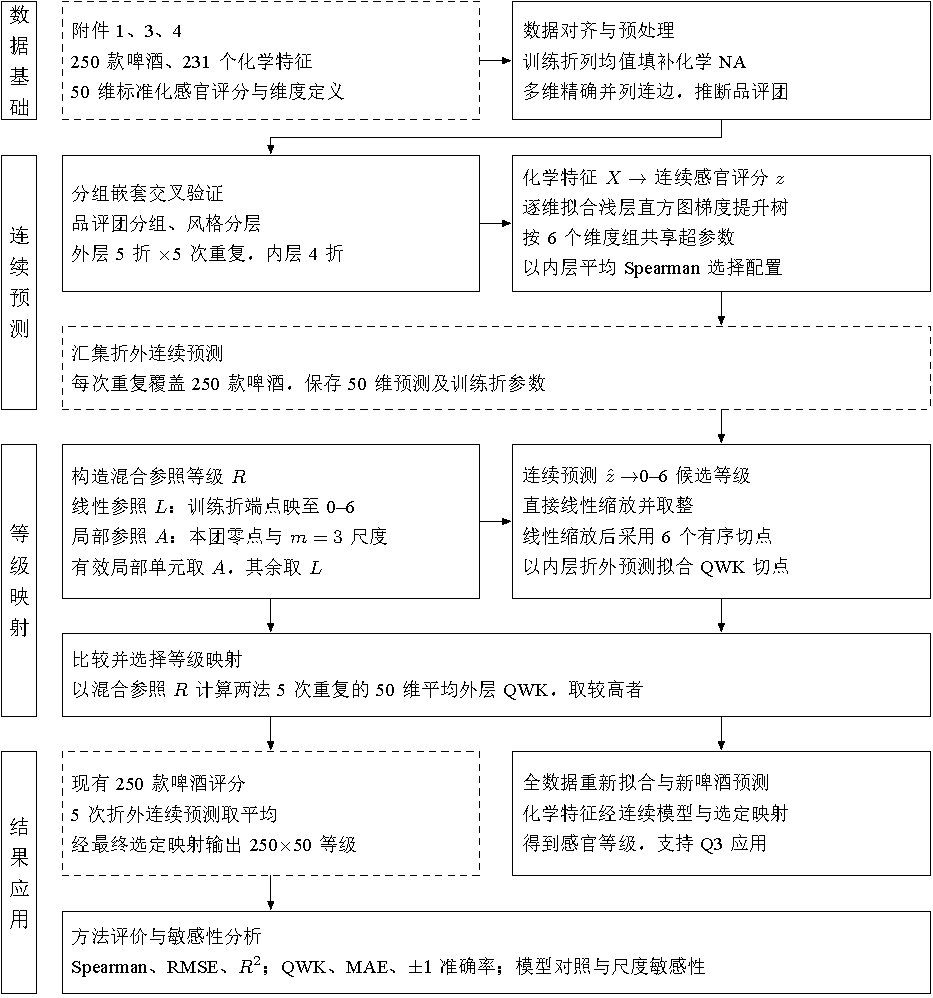
\includegraphics[width=\textwidth]{../figures/q1_methodology_flowchart.pdf}
\caption{问题一方法流程：化学特征与原始评分经日期组嵌套交叉验证得到连续评分与等级预测分布，主输出为分布中位数，第二输出为分位数切点。}
\label{fig:q1-flow}
\end{figure}

对每个感官维度 $d$ 单独训练一个模型 $\hat\mu_{bd}=f_d(X_b)$，以平方损失拟合 $\bar x_{bd}$。
平方损失的最优预测是条件均值，与目标 $\bar x_{bd}$ 的定义一致。
$f_d$ 用 scikit-learn 的 \code{Hist\allowbreak Gradient\allowbreak Boosting\allowbreak Regressor}，是浅层梯度提升树集成。
选用树模型的理由有三点。
第一，Schreurs 等人的论文报告树集成的品评小组测试 $R^2$ 为 0.21 到 0.22，线性回归为 $-4.13$，树集成明显更优。
第二，树只依赖每个特征的顺序，不受 157 个未校准信号列对数底数的影响。
第三，该估计器支持单调约束，也能直接保留缺失值作为敏感性对照。

超参数在每个维度组内共享，以组内平均内层交叉验证的 RMSE 与标准差之比为选择标准。
搜索范围为最大深度 $\{2,3\}$、叶节点最小样本 $\{10,20\}$、学习率 0.05、迭代 $\{100,200,400\}$、$l_2$ 正则 $\{0,1\}$、单调约束开或关。
六个维度组为香气、风味、缺陷、香料啤酒、酸啤酒、基本味口感与总体。
在 250 款啤酒上逐维调参会拟合噪声，因此在 6 个维度组内共享超参数，由内层交叉验证选择。

单调约束来自事先固定的化学知识。
在查看数据之前列出 12 个化合物到感官的配对，其中 11 个符号符合预期，对 6 个直接配对施加约束，包括乙醇到酒精感、苦味单位到苦味、pH 到酸感取负向、乳酸到乳酸感、乙酸到乙酸感、4-乙烯基愈创木酚到酚味。
约束是否开启作为内层交叉验证的超参数，不由外层结果决定。

\subsection{折外残差分布的等级映射与区间估计}

\subsubsection{内层折外残差与等级概率构造}

连续预测需要转为 0 到 6 的等级。
在外层训练集 $\mathcal T$ 上做按日期组分组的 4 折内层交叉验证，得到内层折外预测 $\tilde\mu_{id}$ 与残差 $e_{id}=\bar x_{id}-\tilde\mu_{id}$。
对测试啤酒 $b$，用同一批残差构造预测等级分布：
\begin{equation}\label{eq:q1-p}
\begin{aligned}
p_{bdk}&=\frac{1}{|\mathcal T|}\sum_{i\in\mathcal T}\mathbf 1\!\left\{q(\hat\mu_{bd}+e_{id})=k\right\},\\
F_{bdk}&=\sum_{j\le k}p_{bdj},\qquad k=0,\dots,6 .
\end{aligned}
\end{equation}
式~\eqref{eq:q1-p} 把测试啤酒的预测误差近似为与内层折外残差同分布。
其中 $\mathbf 1\{\cdot\}$ 为指示函数，$p_{bdk}$ 是预测等级为 $k$ 的概率，$F_{bdk}$ 是累积概率。

\subsubsection{分布中位数等级与 90\% 等级区间}

主输出取预测分布的中位数：
\begin{equation}\label{eq:q1-median}
\hat G_{bd}=\min\{k: F_{bdk}\ge 0.5\}.
\end{equation}
主指标是等级 MAE，即平均绝对误差，指预测等级与真实等级之差的绝对值的平均。
在预测分布下使期望等级绝对误差最小的点输出是分布的中位数，因此主输出与主指标匹配。
90\% 等级区间 $[\ell_{bd},u_{bd}]$ 取预测分布的 0.05 与 0.95 分位，$\ell_{bd}=\min\{k:F_{bdk}\ge0.05\}$，$u_{bd}=\min\{k:F_{bdk}\ge0.95\}$。

主输出与四舍五入不同。
零分主导的维度在 0 处截断，残差右偏，等级的中位数不等于 $q(\hat\mu_{bd})$。
完全一致率不作主指标，因为不用化学数据、只输出训练折众数的常数规则完全一致率就有 56.6\%。
主输出、第二输出与主指标都在正式运行前写定。

\subsubsection{分位数切点的补充等级输出}

第二输出取分位数切点，把连续预测 $\hat\mu_{bd}$ 在训练折累积等级频率处的分位数作为切点，输出 $\hat G^{\rm Q}_{bd}=\#\{k:\hat\mu_{bd}\ge c_k\}$，用于保留等级分布的场合。

\subsection{日期组嵌套交叉验证与对照模型设计}

感官评分含品评员之间的系统差异与随机噪声。
同一天品评的啤酒共享出席名单与品评情境，且大多属于同一风格。
随机划分会把同一天品评的啤酒放到训练集与测试集两侧，泄漏同日信息。
因此问题一的交叉验证按日期组隔离，把 37 个品评日期合并成 25 个日期组，每组 5 到 24 款。

表~\ref{tab:q1-setup} 按目标与输入、化学缺失、划分、连续模型、搜索范围、等级与区间、对照与判据七个环节列出正文报告的设置，以及每个设置控制或检验的对象。
软件版本、各折所选参数频数与对照模型的完整搜索网格放附录。

\begin{table}[htbp]
\centering\small
\caption{问题一实验设置与对照}
\label{tab:q1-setup}
\begin{tabular}{p{3.0cm}p{5.4cm}p{4.2cm}}
\toprule
环节 & 正文报告的设置 & 控制或检验什么 \\
\midrule
目标与输入 & 250 款啤酒、231 个化学特征、50 个感官维度；以逐品评员原始评分的每款每维均分为连续目标，均分取整为 0--6 级真值；主模型不输入风格或附件四 & 预测目标、特征与真值同口径 \\
\addlinespace
化学缺失 & 73 个空值在训练折内按列均值填充，测试折不参与预处理 & 填充不泄漏测试信息 \\
\addlinespace
划分 & 37 个日期并为 25 个日期组，按日期组隔离、按风格分层的 5 折 $\times$ 5 次重复，种子 0 到 4，内层同为 4 折 & 同日品评信息不泄漏，调参与报告分开 \\
\addlinespace
连续模型 & 每维一个平方损失 HistGBR，六组内共享超参数，内层按组内平均 RMSE/SD 选参 & 控制模型复杂度 \\
\addlinespace
搜索范围 & 深度 $\{2,3\}$、叶节点 $\{10,20\}$、学习率 0.05、迭代 $\{100,200,400\}$、$l_2$ 正则 $\{0,1\}$、六个单调约束开关由内层选择 & 选参可复现，正文另述迭代下边界检查 \\
\addlinespace
等级与区间 & 内层折外残差构造 0--6 等级概率；分布中位数为主输出，分位数切点为第二输出；90\% 等级区间 & 连续预测转为可交付等级及其不确定性 \\
\addlinespace
对照与判据 & 风格收缩均值为要超越的基线，ElasticNet 检查线性替代，随机森林检查另一种树集成，只用附件四的两阶段方法为对照；主指标等级 MAE，辅助 QWK、完全一致率、$\pm1$ 内比例；按日期组 bootstrap 2,000 次给配对差 95\% 置信区间 & 每个实验为何存在，什么结果支持主张 \\
\bottomrule
\end{tabular}
\end{table}

表~\ref{tab:q1-setup} 的成功标准在运行前声明：主模型等级 MAE 低于风格收缩基线、配对差置信区间上界小于零、且至少 25 个维度逐维 MAE 更低。
指标口径为每次重复合并 250 款折外预测计算，五次再取平均。
最终交付先平均五次概率再取等级，与折外指标口径不同，两者不混用。

\subsection{50 维评分结果、预测误差与区间覆盖}

\subsubsection{整体误差与对照模型比较}

表~\ref{tab:q1-main} 给出主模型与五个关键对照的等级指标。
主模型等级 MAE 为 0.479，风格收缩基线为 0.527，配对差为 $-0.048$，95\% 置信区间为 $[-0.062,-0.034]$，31 个维度逐维 MAE 更低，满足成功标准。

\begin{table}[htbp]
\centering\small
\caption{问题一主结果与关键对照}
\label{tab:q1-main}
\resizebox{\textwidth}{!}{\begin{tabular}{lccccc}
\toprule
模型 & 等级 MAE & 相对主模型的 MAE 差 [95\% CI] & QWK & 完全一致率 & $\pm1$ 内比例 \\
\midrule
风格收缩均值 B1 & 0.527 & $+0.048$ [$0.034$, $0.062$] & 0.095 & 0.559 & 0.931 \\
主模型（化学） & 0.479 & 参照 & 0.290 & 0.581 & 0.950 \\
化学 + 风格 & 0.479 & $-0.0001$ [$-0.0015$, $0.0013$] & 0.289 & 0.580 & 0.950 \\
ElasticNet & 0.481 & $+0.002$ [$-0.010$, $0.013$] & 0.199 & 0.585 & 0.946 \\
随机森林 & 0.472 & $-0.008$ [$-0.015$, $-0.001$] & 0.251 & 0.589 & 0.950 \\
只用附件 C1 & 0.786 & $+0.307$ [$0.271$, $0.341$] & 0.323 & 0.433 & 0.827 \\
\bottomrule
\end{tabular}}
\end{table}

表~\ref{tab:q1-main} 中等级 MAE 为平均绝对误差，QWK 为二次加权 Kappa，完全一致率为预测等级与真实等级相同的单元比例，$\pm1$ 内比例为误差不超过一级的单元比例，单位都是 12,500 个啤酒乘维度单元。

化学加风格一行的结果与主模型相同，回答领域读者最先会问的问题：模型是否只是在识别风格。
只用风格的基线 QWK 为 0.095，在化学特征上再加风格，结果与主模型一致，说明风格信息已由化学谱携带，也支撑问题三只用化学谱给出画像。
随机森林的等级 MAE 为 0.472，低于主模型，但 QWK 为 0.251，低于主模型的 0.290，两者同列呈现，主模型不称各项最优。
只用附件的 C1 按自身规则选定等级映射，端到端等级 MAE 为 0.786，QWK 为 0.323，仍以同一原始等级为真值，其差距主要来自标准化去掉的位置和尺度。

\subsubsection{逐维预测能力与品评信度}

图~\ref{fig:q1-dim} 两栏共用纵轴，50 个维度按六个维度组排列。
左栏为主模型减风格收缩基线的逐维等级 MAE 差，零线区分胜负，标出 31 个胜出维度及各组胜出数。
逐维差只作描述，不把 50 个维度当独立重复求置信区间。
右栏为逐维连续 $R^2$，配同维度的半组信度作短竖线标记。
等级 MAE 受各维度等级分布影响，零分主导的维度 MAE 天然较小，只看左栏会误读维度间差异。
图注写明信度是测量噪声参照，不是严格上限，并注明 $R^2$ 为负的维度。

\begin{figure}[htbp]\centering
\phfig{0.40\textwidth}{左栏为逐维等级 MAE 差（主模型减风格收缩基线），右栏为逐维连续 $R^2$ 与半组信度。}
\caption{逐维增益与可预测性。左栏零线区分主模型与风格收缩基线的逐维胜负，右栏显示逐维连续 $R^2$ 与半组信度。}
\label{fig:q1-dim}
\end{figure}

信度中位数约 0.53，作为噪声参照而非严格性能上限，说明可解释方差的上限就在这一量级。
两半组等级 QWK 为 0.374，是真值本身含抽样噪声的直接证据。
主模型连续 $R^2$ 为 0.184，连续 MAE 为 0.473，连续 Spearman 为 0.360。

\subsubsection{等级分布、高等级收缩与区间覆盖}

表~\ref{tab:q1-rules} 比较四种等级规则。
预测分布中位数与四舍五入的等级 MAE 分别为 0.479 与 0.490，中位数更低且不增加参数。
分位数切点的等级 MAE 为 0.578，高于中位数，但 QWK 为 0.371，高于中位数的 0.290，预测 5 到 6 级的占比为 1.57\%，接近真值的 0.968\%。
主输出服务单款误差最小化，第二输出服务等级分布描述，两者同时交付。

\begin{table}[htbp]
\centering\small
\caption{问题一等级规则比较}
\label{tab:q1-rules}
\resizebox{\textwidth}{!}{\begin{tabular}{lcccc}
\toprule
规则 & 等级 MAE & QWK & 完全一致率 & 预测 5--6 级占比 \\
\midrule
常数等级（训练折众数） & 0.549 & $-0.006$ & 0.566 & 0\% \\
四舍五入 & 0.490 & 0.293 & 0.565 & 0.04\% \\
预测分布中位数（主输出） & 0.479 & 0.290 & 0.581 & 0.02\% \\
分位数切点（第二输出） & 0.578 & 0.371 & 0.531 & 1.57\% \\
\bottomrule
\end{tabular}}
\end{table}

保持等级分布提高 QWK，但单款啤酒的误差变大。
原因是模型只解释了一部分方差，最优的单点预测必然向中间收缩。
要让等级分布与真值一致，就得把部分啤酒推离它最可能的等级。
这一取舍由表~\ref{tab:q1-rules} 与图~\ref{fig:q1-grade} 共同呈现。

图~\ref{fig:q1-grade} 左栏为真值、主输出、第二输出的 0 到 6 级频率，右栏为按真实等级分层的主输出召回率。
$\pm1$ 内比例约 95\% 会掩盖高等级漏判，本图回答这一疑虑。
主输出几乎不给出 5 到 6 级，5 级真值 112 个单元、6 级 9 个单元的召回率接近零，误差集中在相邻等级。
第二输出给出 1.57\% 的 5 到 6 级，更接近真值。

\begin{figure}[htbp]\centering
\phfig{0.40\textwidth}{左栏为真值、主输出、第二输出的 0--6 级频率，右栏为按真实等级分层的主输出召回率。}
\caption{误差集中的等级。左栏显示三种等级频率，右栏显示主输出按真实等级分层的召回率，图注注明每栏分母。}
\label{fig:q1-grade}
\end{figure}

90\% 等级区间覆盖 97.2\%，平均宽度 1.97 级，略宽于名义值，来自等级的离散性与折外残差的保守性。

\subsubsection{交付评分示例}

赛题要求给出评分结果，表~\ref{tab:q1-delivery} 展示交付物本身。
选款规则事先固定，在 Pils/Lager、Tripel、Kriek 三个风格中各取原始评分记录数最多的一款，与问题三的风格相连。
行为 15 个属性，列为三款啤酒的 Aroma 与 Flavour，共 6 列。
单元格写交付等级与 90\% 区间，再附实测等级。
全部 250 款作为机器可读补充文件交付。

\begin{table}[htbp]
\centering\small
\caption{交付评分示例：三款啤酒的 15 个属性}
\label{tab:q1-delivery}
\resizebox{\textwidth}{!}{\begin{tabular}{lcccccc}
\toprule
属性 & \multicolumn{2}{c}{Pils/Lager} & \multicolumn{2}{c}{Tripel} & \multicolumn{2}{c}{Kriek} \\
 & Aroma & Flavour & Aroma & Flavour & Aroma & Flavour \\
\midrule
malt\_all & \ph & \ph & \ph & \ph & \ph & \ph \\
\addlinespace
\multicolumn{7}{l}{\small 单元格格式为交付等级 [90\% 区间] / 实测等级，取自最终交付口径 $G_{hat}$，与折外指标口径不同。} \\
\addlinespace
\multicolumn{7}{l}{\small 占位单元格由 Coding 从 \code{q1\_final\_scores.csv} 导出，三款啤酒按选款规则在三个风格中取评分记录数最多者。} \\
\bottomrule
\end{tabular}}
\end{table}

\subsection{缺失值处理、评分目标与等级规则的敏感性分析}

敏感性分析共八项，其中七项的等级 MAE 配对差置信区间含 0，交付等级变化不超过 5.2\%。
训练目标改为训练折内估计的啤酒效应、化学缺失的三种替代填充、barnyard 的排除、四个综合指标的删除、附件八冲突单元替换、单调约束全开或全关，都不改变主要结论。
网格扩展检查在重复 0 上把迭代下界扩展到 10 到 200，外层连续 MAE 与 $R^2$ 不变，Spearman 低 0.019，未改善外层预测，主网格保持不变。
只用附件的对照 C1，其零点还原的中间结果见表~\ref{tab:prep-reference}，端到端结果见表~\ref{tab:q1-main}。
